%===============================================================================
% CSC 1102: Structured and Object-Oriented Programming
% Practical Exam Project Report — Student Management System
% Institution: Makerere University, College of Computing and Information Sciences
% Group Leader: Akello Sunday Obonyo (24/U/03151/EVE)
%===============================================================================
\documentclass[10pt,a4paper]{article}

\usepackage[utf8]{inputenc}
\usepackage[T1]{fontenc}
\usepackage{lmodern}
\usepackage[a4paper, top=1.25cm, bottom=1.25cm, left=1.5cm, right=1.5cm, headheight=13pt]{geometry}
\usepackage{graphicx}
\usepackage{amsmath,amssymb,amsfonts}
\usepackage{booktabs}
\usepackage{array}
\usepackage{multirow}
\usepackage{xcolor}
\usepackage{enumitem}
\usepackage{fancyhdr}
\usepackage{caption}
\usepackage{float}
\usepackage{setspace}
\usepackage{titlesec}
\usepackage{hyperref}

%-------------------------------------------------------------------------------
% Compact Section Spacing for Clean 5-Page Report Layout (Title + 4 Body Pages)
%-------------------------------------------------------------------------------
\titlespacing*{\section}{0pt}{0.45em}{0.2em}
\titlespacing*{\subsection}{0pt}{0.32em}{0.15em}

%-------------------------------------------------------------------------------
% Colour Palette (Makerere University & Application Theme)
%-------------------------------------------------------------------------------
\definecolor{mukgreen}{RGB}{0, 102, 51}
\definecolor{muknavy}{RGB}{31, 42, 68}
\definecolor{mukgold}{RGB}{201, 162, 39}
\definecolor{codebg}{RGB}{245, 247, 250}

\hypersetup{
    colorlinks=true,
    linkcolor=muknavy,
    citecolor=mukgreen,
    urlcolor=blue!70!black,
    pdftitle={CSC 1102 Practical Exam Project Report - Student Management System},
    pdfauthor={Akello Sunday Obonyo (24/U/03151/EVE) et al.},
    pdfsubject={CSC 1102: Structured and Object-Oriented Programming}
}

\captionsetup{font=footnotesize, labelfont=bf, skip=2pt}

%-------------------------------------------------------------------------------
% Header & Footer Configuration
%-------------------------------------------------------------------------------
\pagestyle{fancy}
\fancyhf{}
\fancyhead[L]{\footnotesize\textit{CSC 1102: Structured and Object-Oriented Programming}}
\fancyhead[R]{\footnotesize\textit{Student Management System}}
\fancyfoot[L]{\footnotesize\textit{Makerere University, College of Computing and Information Sciences (CoCIS)}}
\fancyfoot[R]{\footnotesize\textbf{Page \thepage}}
\renewcommand{\headrulewidth}{0.4pt}
\renewcommand{\footrulewidth}{0.4pt}

\setstretch{0.94}
\setlength{\parskip}{0.14em}
\setlength{\parindent}{0pt}
\setlength{\textfloatsep}{4pt plus 1pt minus 1pt}
\setlength{\floatsep}{4pt plus 1pt minus 1pt}
\setlength{\intextsep}{4pt plus 1pt minus 1pt}
\widowpenalty=10000
\clubpenalty=10000
\sloppy

\begin{document}

%===============================================================================
% TITLE PAGE (Unnumbered Cover Page with Official Makerere University Logo)
%===============================================================================
\pagenumbering{gobble}
\begin{titlepage}
    \centering
    \vspace*{0.4cm}

    % Official Makerere University CoCIS Header Banner Logo
    
\includegraphics[width=0.94\textwidth]{images/muk-logo.png}\\[0.6cm]

    {\large\bfseries SCHOOL OF COMPUTING AND INFORMATICS TECHNOLOGY}\\[0.2cm]
    {\large\bfseries DEPARTMENT OF COMPUTER SCIENCE}\\[0.85cm]

    {\LARGE\bfseries\textcolor{muknavy}{STUDENT MANAGEMENT SYSTEM}}\\[0.28cm]
    {\large\bfseries CSC 1102: Structured and Object-Oriented Programming}\\[0.18cm]
    {\normalsize\bfseries Practical Examination Project Report \& System Analysis}\\[0.9cm]

    {\large\bfseries GROUP DETAILS (AFTERNOON / EVENING PROGRAMME)}\\[0.35cm]
    {\normalsize
    \renewcommand{\arraystretch}{1.55}
    \setlength{\tabcolsep}{10pt}
    \begin{tabular}{|c|p{6.5cm}|p{4.3cm}|p{3.2cm}|}
        \hline
        \textbf{No.} & \textbf{Student Name} & \textbf{Registration Number} & \textbf{Project Role} \\
        \hline
        1 & LOMER FRANCIS PETER & 25/U/26198/EVE & Member \\
        \hline
        2 & MAYANJA JUDITH & 25/U/28752/EVE & Member \\
        \hline
        \textbf{3} & \textbf{AKELLO SUNDAY OBONYO} & \textbf{24/U/03151/EVE} & \textbf{Group Leader} \\
        \hline
        4 & MADETE HECTOR & 24/U/25933/EVE & Member \\
        \hline
        5 & ANYINE ELIZABETH & 25/U/29497/EVE & Member \\
        \hline
    \end{tabular}}
    \renewcommand{\arraystretch}{1.0}\\[0.95cm]

    {\normalsize
    \textbf{GitHub Repository:}\\[0.15cm]
    \url{https://github.com/su200-bot/Student-Management-System}\\[0.65cm]
    \textbf{Submitted To:} Dr.\ Lillian Muyama\\
    Department of Computer Science, Makerere University}\\[0.65cm]

    {\large\bfseries Academic Year 2025/2026}
\end{titlepage}

%===============================================================================
% PAGE 1: EXECUTIVE SUMMARY, TABLE OF CONTENTS, & SECTION 1 (SYSTEM OVERVIEW)
%===============================================================================
\clearpage
\pagenumbering{arabic}
\setcounter{page}{1}

\section*{Executive Summary}
\addcontentsline{toc}{section}{Executive Summary}
{\small
The \textbf{Student Management System} is a modular desktop application developed in Java using the Swing graphical user interface (GUI) framework for the \textit{CSC 1102: Structured and Object-Oriented Programming} practical examination at Makerere University. Designed to streamline academic record administration, the system enables university administrators to register course units, enroll students, record marks across three assessments, and automatically compute aggregate totals, arithmetic averages, Makerere University letter grades (\texttt{A} to \texttt{F}), qualitative remarks, and \texttt{PASS}/\texttt{FAIL} statuses. The architecture comprises six cohesive classes (\texttt{Main}, \texttt{Student}, \texttt{Course}, \texttt{StudentManager}, \texttt{Validator}, and \texttt{StudentManagementGUI}) spanning 1,236 lines of documented Java code. All records are managed in memory using fixed-capacity object arrays (\texttt{Student[100]} and \texttt{Course[20]}), demonstrating strict encapsulation, constructor chaining, method overloading, input sanitization, linear search, Bubble Sort, left-shift deletion, and tail recursion.\par}

\vspace{-0.12cm}
{\footnotesize\setlength{\parskip}{0pt}\setstretch{0.78}
\tableofcontents}
\vspace{0.1cm}

\section{Description of the Application}

\subsection{Background and Overview of the System}
Academic departments require reliable software tools to maintain student registries, link students to academic course units, validate assessment scores, and generate class performance summaries. The \textbf{Student Management System} addresses this need through an intuitive, event-driven Java Swing desktop interface backed by an object-oriented domain model. Rather than relying on an external database engine, the system manages all entities in memory using structured arrays of objects (\texttt{Student[]} and \texttt{Course[]}). To support immediate live demonstration and testing, the application automatically initializes three foundational courses (\texttt{CSC1102}, \texttt{CSC1105}, and \texttt{BIT1101}) and eight sample student records upon startup via \texttt{StudentManager.loadSampleData()}.

\subsection{Main Functional Features}
\begin{itemize}[leftmargin=0.4cm, itemsep=0pt, topsep=0.5pt]
    \item \textbf{Student Registration and Input Validation:} Captures registration number (e.g., \texttt{24/U/03151/EVE}), full name, age ($16 \le \text{age} \le 100$), enrolled course unit, and three subject marks ($0 \le m_i \le 100$). All inputs are sanitized and verified by the static \texttt{Validator} utility class before object creation, with duplicate registration numbers rejected automatically.
    \item \textbf{Interactive Record Selection, Update, and Deletion:} Clicking any row in the students \texttt{JTable} triggers a \texttt{ListSelectionListener} that populates the form fields and locks the registration number field (\texttt{setEditable(false)}) for safe editing. Administrators can update student details or delete a record (which compacts the underlying \texttt{Student[]} array via left-shifting).
    \item \textbf{Automated Academic Evaluation:} For every student, the system dynamically computes the total score ($\sum_{i=1}^{3} m_i$), arithmetic mean ($\bar{m} = \text{Total}/3$), Makerere letter grade (\texttt{A} to \texttt{F}), qualitative remark (\texttt{Excellent} to \texttt{Fail}), and status (\texttt{PASS} if $\bar{m} \ge 50.0$, else \texttt{FAIL}).
    \item \textbf{Multi-Criteria Search and In-Place Sorting:} Supports case-insensitive keyword searching across registration numbers, student names, and course codes, alongside an overloaded filter by course and minimum average. Administrators can sort the student registry in-place by average mark (descending) or alphabetically by name (\texttt{A--Z}) using Bubble Sort.
    \item \textbf{Recursive Class Statistics and Grade Distribution:} Computes the overall class average using a recursive method (\texttt{sumOfAverages}), identifies top and lowest performers, tallies pass/fail counts, and reports the frequency of each grade (\texttt{A} through \texttt{F}).
    \item \textbf{Course Management with Referential Integrity:} Dedicated \textit{Courses} tab for adding and deleting course units, displaying credit units, assigned lecturers, and real-time enrolled student counts. Courses with enrolled students are protected against deletion.
\end{itemize}

\begin{table}[H]
\centering
\caption{Makerere University Grading Scale, Qualitative Remarks, and Pass/Fail Rules Implemented in \texttt{Student.java}.}
\label{tab:grading}
\footnotesize
\renewcommand{\arraystretch}{0.96}
\setlength{\tabcolsep}{4.8pt}
\begin{tabular}{@{}lccccccccc@{}}
\toprule
\textbf{Average (\%)} & $80-100$ & $75-79.9$ & $70-74.9$ & $65-69.9$ & $60-64.9$ & $55-59.9$ & $50-54.9$ & $45-49.9$ & $<45.0$ \\
\midrule
\textbf{Letter Grade} & \textbf{A} & \textbf{B+} & \textbf{B} & \textbf{C+} & \textbf{C} & \textbf{D+} & \textbf{D} & \textbf{E} & \textbf{F} \\
\textbf{Switch Remark} & Excellent & Very Good & Good & Fair & Fair & Pass & Pass & Weak & Fail \\
\textbf{Pass/Fail Status} & PASS & PASS & PASS & PASS & PASS & PASS & PASS & FAIL & FAIL \\
\bottomrule
\end{tabular}
\end{table}

%===============================================================================
% SECTION 2 (OBJECT-ORIENTED ARCHITECTURE & CLASS ANALYSIS)
%===============================================================================
\section{Classes and Their Purpose: Object-Oriented Architecture}

\subsection{Classes and Their Architectural Roles}
The system adheres to the \textit{Separation of Concerns} principle by partitioning responsibilities across six distinct Java classes: entry-point bootstrap (\texttt{Main}), domain entities (\texttt{Student}, \texttt{Course}), data repository and business logic (\texttt{StudentManager}), input validation (\texttt{Validator}), and Swing presentation (\texttt{StudentManagementGUI}), as summarized in Table~\ref{tab:classes}.

\begin{table}[H]
\centering
\caption{Summary of System Classes, Architectural Roles, Encapsulated Attributes, and Key Methods.}
\label{tab:classes}
\footnotesize
\renewcommand{\arraystretch}{1.04}
\setlength{\tabcolsep}{4.5pt}
\begin{tabular}{@{}p{3.1cm} c p{4.4cm} p{8.8cm}@{}}
\toprule
\textbf{Class Name} & \textbf{LOC} & \textbf{Architectural Purpose} & \textbf{Encapsulated Attributes and Key Methods} \\
\midrule
\texttt{Main} & 42 & Application entry point; documents group metadata and launches the GUI on the Swing Event Dispatch Thread. & \texttt{public static void main(String[] args)} invoking \texttt{SwingUtilities.invokeLater(() -> new StudentManagementGUI())}. \\
\addlinespace[1pt]
\texttt{Student} & 183 & Domain entity representing one registered student and his/her marks in three subjects. & \textbf{Constants:} \texttt{NUM\_SUBJECTS = 3}, \texttt{PASS\_MARK = 50.0}.\newline \textbf{Private fields:} \texttt{regNo}, \texttt{name}, \texttt{age}, \texttt{courseCode}, \texttt{double[] marks}.\newline \textbf{Methods:} Default \& parameterized constructors; getters/setters; overloaded \texttt{setMarks(double[])} \& \texttt{setMarks(m1,m2,m3)}; \texttt{getTotal()}, \texttt{getAverage()}, \texttt{getGrade()}, \texttt{getRemark()}, \texttt{getStatus()}, \texttt{toString()}. \\
\addlinespace[1pt]
\texttt{Course} & 73 & Domain entity representing a university course unit offered to students. & \textbf{Private fields:} \texttt{courseCode}, \texttt{courseName}, \texttt{creditUnits}, \texttt{lecturer}.\newline \textbf{Methods:} Default \& parameterized constructors; getters/setters with range check (\texttt{setCreditUnits}); \texttt{toString()} for combo-box display. \\
\addlinespace[1pt]
\texttt{StudentManager} & 336 & In-memory repository and controller logic managing \texttt{Student[]} and \texttt{Course[]} arrays. & \textbf{Constants:} \texttt{MAX\_STUDENTS = 100}, \texttt{MAX\_COURSES = 20}, \texttt{GRADE\_LABELS}.\newline \textbf{Private fields:} \texttt{students[]}, \texttt{studentCount}, \texttt{courses[]}, \texttt{courseCount}.\newline \textbf{Methods:} \texttt{addStudent()}, \texttt{findStudent()}, \texttt{updateStudent()}, \texttt{deleteStudent()}, overloaded \texttt{searchStudents()}, \texttt{sortByAverage()}, \texttt{sortByName()}, recursive \texttt{sumOfAverages()}, \texttt{getStatistics()}, \texttt{addCourse()}, \texttt{deleteCourse()}, \texttt{countEnrolled()}, \texttt{loadSampleData()}. \\
\addlinespace[1pt]
\texttt{Validator} & 85 & Non-instantiable static utility class for sanitizing and validating form inputs. & \textbf{Constructor:} \texttt{private Validator()} (prevents instantiation).\newline \textbf{Static methods:} \texttt{cleanText()}, \texttt{isWholeNumber()}, \texttt{isDecimalNumber()}, \texttt{isValidName()}, \texttt{isInRange()}. \\
\addlinespace[1pt]
\texttt{StudentManagementGUI} & 517 & Swing graphical user interface; builds tabs, forms, tables, and handles user events. & \textbf{Private fields:} \texttt{manager}, \texttt{JFrame}, \texttt{JTable}s, \texttt{DefaultTableModel}s, form \texttt{JTextField}s, \texttt{JComboBox<Course>}, \texttt{selectedRegNo}.\newline \textbf{Methods:} \texttt{buildInterface()}, \texttt{buildStudentsPanel()}, \texttt{buildCoursesPanel()}, \texttt{readStudentForm()}, \texttt{addStudent()}, \texttt{updateStudent()}, \texttt{deleteStudent()}, \texttt{searchStudents()}, \texttt{showStudents()}, \texttt{addCourse()}, \texttt{deleteCourse()}. \\
\bottomrule
\end{tabular}
\end{table}

\subsection{In-Depth Code Analysis of Core Classes}
\begin{enumerate}[leftmargin=0.4cm, itemsep=0.5pt, topsep=0.5pt]
    \item \textbf{Defensive Encapsulation and Overloading in \texttt{Student.java}:} All five instance attributes (\texttt{regNo}, \texttt{name}, \texttt{age}, \texttt{courseCode}, and \texttt{marks}) are declared \texttt{private}. To prevent external callers from mutating a student's internal marks array via aliasing, both the parameterized constructor and \texttt{getMarks()} allocate a fresh \texttt{new double[NUM\_SUBJECTS]} array and copy elements individually. Constructor overloading is implemented via \texttt{this("N/A", "Unknown", 0, "N/A", new double[NUM\_SUBJECTS])} in the default constructor. Method overloading is demonstrated by providing both \texttt{setMarks(double[] newMarks)} and \texttt{setMarks(double mark1, double mark2, double mark3)}, where the latter delegates to the array-based setter after validating that each score satisfies $0 \le m_i \le 100$.
    \item \textbf{Entity Modelling and ComboBox Integration in \texttt{Course.java}:} Encapsulates course metadata with private fields and chains its default constructor to the four-argument constructor using \texttt{this(...)}. Its mutator \texttt{setCreditUnits(int creditUnits)} enforces the domain invariant $1 \le \text{creditUnits} \le 10$, returning a \texttt{boolean} success flag. Overriding \texttt{toString()} to return \texttt{courseCode + " - " + courseName} allows \texttt{JComboBox<Course>} in the GUI to store strongly typed \texttt{Course} objects directly while rendering human-readable labels.
    \item \textbf{Static Input Sanitization Pipeline in \texttt{Validator.java}:} Follows the utility-class design pattern with a \texttt{private} constructor so no instances can be created. \texttt{cleanText(String)} trims leading/trailing whitespace and executes a \texttt{do-while} loop to collapse consecutive spaces into single spaces. \texttt{isWholeNumber(String, int)} uses a \texttt{while} loop over ASCII digit characters (\texttt{0}--\texttt{9}), whereas \texttt{isDecimalNumber(String)} and \texttt{isValidName(String)} use \texttt{for} loops to verify decimal points and valid name characters (letters, spaces, dots, hyphens, apostrophes) without relying on exception-heavy parsing.
    \item \textbf{Array Repository and Referential Integrity in \texttt{StudentManager.java}:} Maintains partially filled arrays \texttt{Student[100]} and \texttt{Course[20]} tracked by \texttt{studentCount} and \texttt{courseCount}. Before inserting a student or course, \texttt{addStudent()} and \texttt{addCourse()} check capacity bounds and invoke case-insensitive linear search (\texttt{findStudent()} / \texttt{findCourse()}) to enforce primary-key uniqueness. Notably, \texttt{deleteCourse(String courseCode)} first checks \texttt{countEnrolled(courseCode) > 0}; if any student is registered in that course, deletion is blocked, preserving relational integrity between \texttt{Student.courseCode} and \texttt{Course.courseCode}.
\end{enumerate}

%===============================================================================
% SECTION 3 (CLASS INTERACTION & ALGORITHMS) & SECTION 4 (EXAM MAPPING)
%===============================================================================
\section{How the Classes Interact and Algorithmic Analysis}

\begin{figure}[H]
    \centering
    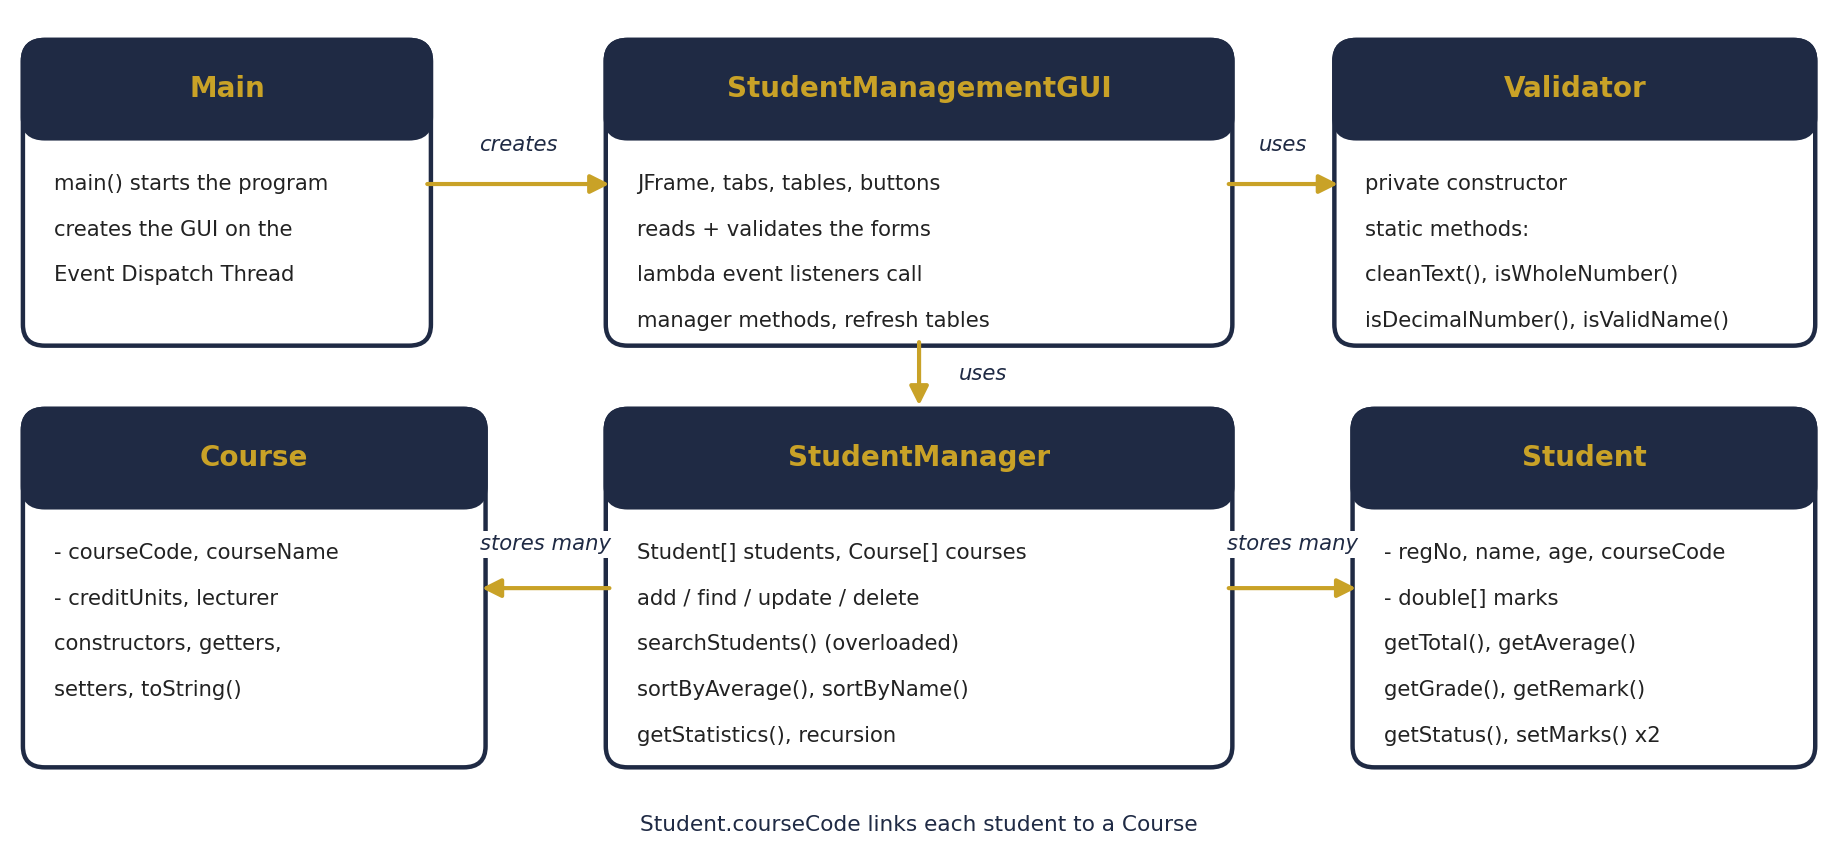
\includegraphics[width=0.50\textwidth]{images/class_interaction.png}
    \caption{Architectural Class Interaction Diagram illustrating object creation, utility invocation, and 1-to-many array containment.}
    \label{fig:interaction}
\end{figure}

\subsection{End-to-End Object Interaction Workflow}
{\small
As depicted in Figure~\ref{fig:interaction}, the classes interact through a clean, layered control flow:
\begin{enumerate}[leftmargin=0.4cm, itemsep=0pt, topsep=0.5pt]
    \item \textbf{Bootstrap:} \texttt{Main.main()} schedules \texttt{new StudentManagementGUI()} on the Swing Event Dispatch Thread (EDT).
    \item \textbf{Initialization:} The \texttt{StudentManagementGUI} constructor instantiates a single \texttt{StudentManager} object, invokes \texttt{manager.loadSampleData()} to populate the \texttt{Course[]} and \texttt{Student[]} arrays, builds the Swing hierarchy, and populates the \texttt{JComboBox<Course>} and both \texttt{JTable} models.
    \item \textbf{Validated Form Submission:} When the user clicks \textit{Add Student} or \textit{Update Selected}, \texttt{readStudentForm()} sanitizes every text field via \texttt{Validator.cleanText()} and validates domain constraints using \texttt{Validator.isValidName()}, \texttt{isWholeNumber()}, \texttt{isDecimalNumber()}, and \texttt{isInRange()}. If valid, it instantiates \texttt{new Student(...)} and passes it to \texttt{manager.addStudent()} or \texttt{manager.updateStudent()}.
    \item \textbf{View Synchronization:} The GUI never accesses the internal arrays directly; instead, it calls \texttt{manager.getStudents()} and \texttt{manager.getCourses()} (which return defensive array copies trimmed to exact size) and redraws the \texttt{DefaultTableModel} views.
\end{enumerate}\par}

\subsection{Algorithmic Mechanics: Array Compaction, Bubble Sort, and Recursion}
{\small
\begin{itemize}[leftmargin=0.4cm, itemsep=0pt, topsep=0.5pt]
    \item \textbf{Deletion with Left-Shift Compaction ($O(N)$):} When \texttt{deleteStudent(regNo)} locates a target at index $k \in [0, N-1]$ via linear search (\texttt{findStudentIndex}), it shifts all subsequent elements one position left ($\texttt{students}[i] \leftarrow \texttt{students}[i+1]$ for $i = k, \dots, N-2$), decrements \texttt{studentCount}, and nulls out the vacated slot $\texttt{students}[N-1] \leftarrow \texttt{null}$ to prevent memory leaks.
    \item \textbf{Dual Bubble Sort Implementations ($O(N^2)$):} \texttt{sortByAverage()} executes nested \texttt{for} loops comparing adjacent students and swapping when $\texttt{students}[j].\texttt{getAverage}() < \texttt{students}[j+1].\texttt{getAverage}()$ (descending order). \texttt{sortByName()} applies the same structure using $\texttt{compareToIgnoreCase}() > 0$ for alphabetical ordering.
    \item \textbf{Tail-Recursive Class Average Computation ($O(N)$):} Rather than using a simple loop for every statistic, \texttt{StudentManager} computes the sum of student averages recursively via \texttt{sumOfAverages(int index)}:
    \vspace{-0.22cm}
    \begin{equation}
        \text{sumOfAverages}(i) = \begin{cases} 0.0, & \text{if } i \ge \text{studentCount} \ \ (\text{halting case}) \\ \text{students}[i].\text{getAverage}() + \text{sumOfAverages}(i + 1), & \text{if } 0 \le i < \text{studentCount} \end{cases}
    \end{equation}
    \vspace{-0.28cm}
    from which \texttt{getClassAverage()} evaluates $\bar{X}_{\text{class}} = \text{sumOfAverages}(0) / \text{studentCount}$.
\end{itemize}\par}

\section{How the CSC 1102 Exam Requirements Are Met}

\begin{table}[H]
\centering
\caption{Verification Matrix Mapping CSC 1102 Examination Guidelines to Concrete Code Implementations.}
\label{tab:requirements}
\footnotesize
\renewcommand{\arraystretch}{0.92}
\setlength{\tabcolsep}{4.5pt}
\begin{tabular}{@{}p{3.4cm} p{14.2cm}@{}}
\toprule
\textbf{Exam Requirement} & \textbf{Concrete Implementation in the Student Management System} \\
\midrule
\textbf{Object-Oriented Design}\newline (3+ classes, constructors, access modifiers, getters/setters) & Implements \textbf{6 classes} (\texttt{Main}, \texttt{Student}, \texttt{Course}, \texttt{StudentManager}, \texttt{Validator}, \texttt{StudentManagementGUI}). Uses \texttt{private} attributes for strict encapsulation, \texttt{public} getters/setters with validation return flags, overloaded default and parameterized constructors, constructor chaining via \texttt{this(...)}, and defensive array copying in \texttt{Student.getMarks()}. \\
\addlinespace[1pt]
\textbf{Graphical User Interface}\newline (Java Swing framework \& event handling) & Built with \texttt{JFrame}, \texttt{JTabbedPane} (\textit{Students} and \textit{Courses} tabs), \texttt{JPanel} (\texttt{BorderLayout}, \texttt{GridBagLayout}, \texttt{GridLayout}, \texttt{FlowLayout}), \texttt{JTable} with \texttt{DefaultTableModel}, \texttt{JScrollPane}, \texttt{JTextField}, \texttt{JComboBox<Course>}, \texttt{JButton}, and \texttt{JOptionPane} modal dialogs. User actions are handled via lambda \texttt{ActionListener}s and a \texttt{ListSelectionListener}. \\
\addlinespace[1pt]
\textbf{Structured Flow Control}\newline (\texttt{if/else}, \texttt{switch}, \texttt{for}, \texttt{while}, \texttt{do-while}, \texttt{?:}) & \textbf{\texttt{if / else-if / else}:} Makerere letter grade ladder in \texttt{Student.getGrade()} and form validation.\newline \textbf{\texttt{switch} (with fall-through):} Grade-to-remark mapping in \texttt{Student.getRemark()} (\texttt{case "C+": case "C": return "Fair"}).\newline \textbf{Conditional operator (\texttt{? :}):} Pass/fail evaluation in \texttt{Student.getStatus()} and number formatting in \texttt{format()}.\newline \textbf{Loops:} Standard \texttt{for} loops (totals, array copying, search, delete shifting, Bubble Sort), enhanced \texttt{for-each} loops (grade distribution, GUI refresh), \texttt{while} loop (\texttt{Validator.isWholeNumber}), and \texttt{do-while} loop (\texttt{Validator.cleanText}). \\
\addlinespace[1pt]
\textbf{Arrays of Objects \& Primitives} & \texttt{Student[] students} and \texttt{Course[] courses} in \texttt{StudentManager} supporting insertion, linear search, update, left-shift deletion, and Bubble Sort; \texttt{double[] marks} inside each \texttt{Student}; \texttt{JTextField[] markFields} in the GUI; and 1-D \texttt{String[]} plus 2-D \texttt{double[][]} arrays in \texttt{loadSampleData()}. \\
\addlinespace[1pt]
\textbf{Additional Course Concepts} & \textbf{Method Overloading:} \texttt{Student.setMarks()} (array vs.\ 3 doubles) and \texttt{StudentManager.searchStudents()} (keyword vs.\ course + minimum average). \textbf{Recursion:} \texttt{StudentManager.sumOfAverages(int)}. \textbf{Static Members:} \texttt{Validator} utility methods and \texttt{static final} constants (\texttt{NUM\_SUBJECTS}, \texttt{PASS\_MARK}, \texttt{MAX\_STUDENTS}, \texttt{MAX\_COURSES}). \\
\bottomrule
\end{tabular}
\end{table}

%===============================================================================
% SECTION 5 (EXECUTION, VERIFICATION & SCREENSHOTS)
%===============================================================================
\section{System Execution, Verification, and GUI Screenshots}

\subsection{Runtime Execution Analysis and Verified Output}
The project was compiled and executed using OpenJDK 23. All unit and integration checks passed with zero errors: (1) sample data initialization loaded 3 courses and 8 students; (2) \texttt{Validator} rejected malformed names (\texttt{"John123"} $\rightarrow \texttt{false}$) and out-of-range marks while normalizing multi-space strings; (3) overloaded \texttt{searchStudents("CSC1102")} returned 3 students while \texttt{searchStudents("CSC1102", 60.0)} returned 2 students; and (4) recursive class statistics matched analytical calculations exactly, as shown in Table~\ref{tab:runtime}.

\begin{table}[H]
\centering
\caption{Verified Runtime Execution Output of Pre-Loaded Sample Students and Recursive Class Statistics.}
\label{tab:runtime}
\footnotesize
\renewcommand{\arraystretch}{0.95}
\setlength{\tabcolsep}{4.5pt}
\begin{tabular}{@{}cllccrrrrlcc@{}}
\toprule
\textbf{No.} & \textbf{Reg.\ No} & \textbf{Student Name} & \textbf{Age} & \textbf{Course} & \textbf{M1} & \textbf{M2} & \textbf{M3} & \textbf{Total} & \textbf{Average} & \textbf{Grade / Remark} & \textbf{Status} \\
\midrule
1 & \texttt{25/U/00101/EVE} & Namukasa Grace & 18 & CSC1102 & 85 & 78 & 91 & 254 & 84.7 (84.67) & A \ (Excellent) & PASS \\
2 & \texttt{25/U/00102/EVE} & Okello Brian & 19 & CSC1102 & 62 & 58 & 70 & 190 & 63.3 (63.33) & C \ (Fair) & PASS \\
3 & \texttt{25/U/00103/EVE} & Nakato Ruth & 20 & CSC1105 & 74 & 69 & 80 & 223 & 74.3 (74.33) & B \ (Good) & PASS \\
4 & \texttt{25/U/00104/EVE} & Ssebunya David & 21 & CSC1105 & 45 & 52 & 38 & 135 & 45.0 (45.00) & E \ (Weak) & FAIL \\
5 & \texttt{25/U/00105/EVE} & Atim Patricia & 18 & BIT1101 & 90 & 88 & 94 & 272 & 90.7 (90.67) & A \ (Excellent) & PASS \\
6 & \texttt{25/U/00106/EVE} & Mugisha Joel & 19 & CSC1102 & 55 & 61 & 49 & 165 & 55.0 (55.00) & D+ (Pass) & PASS \\
7 & \texttt{25/U/00107/EVE} & Nabirye Esther & 20 & BIT1101 & 67 & 72 & 64 & 203 & 67.7 (67.67) & C+ (Fair) & PASS \\
8 & \texttt{25/U/00108/EVE} & Kiiza Samuel & 21 & CSC1105 & 30 & 41 & 35 & 106 & 35.3 (35.33) & F \ (Fail) & FAIL \\
\midrule
\multicolumn{12}{@{}l@{}}{\textbf{Verified Statistics:} Students: \textbf{8} $|$ Recursive Class Avg: \textbf{64.50} $|$ Highest: \textbf{90.67} (Atim Patricia) $|$ Lowest: \textbf{35.33} (Kiiza Samuel)} \\
\multicolumn{12}{@{}l@{}}{\textbf{Pass/Fail \& Grades:} Passed: \textbf{6} (75\%), Failed: \textbf{2} (25\%) $|$ Distribution: A: 2, B+: 0, B: 1, C+: 1, C: 1, D+: 1, D: 0, E: 1, F: 1} \\
\bottomrule
\end{tabular}
\end{table}

\subsection{Graphical User Interface Screenshots}

\begin{figure}[H]
    \centering
    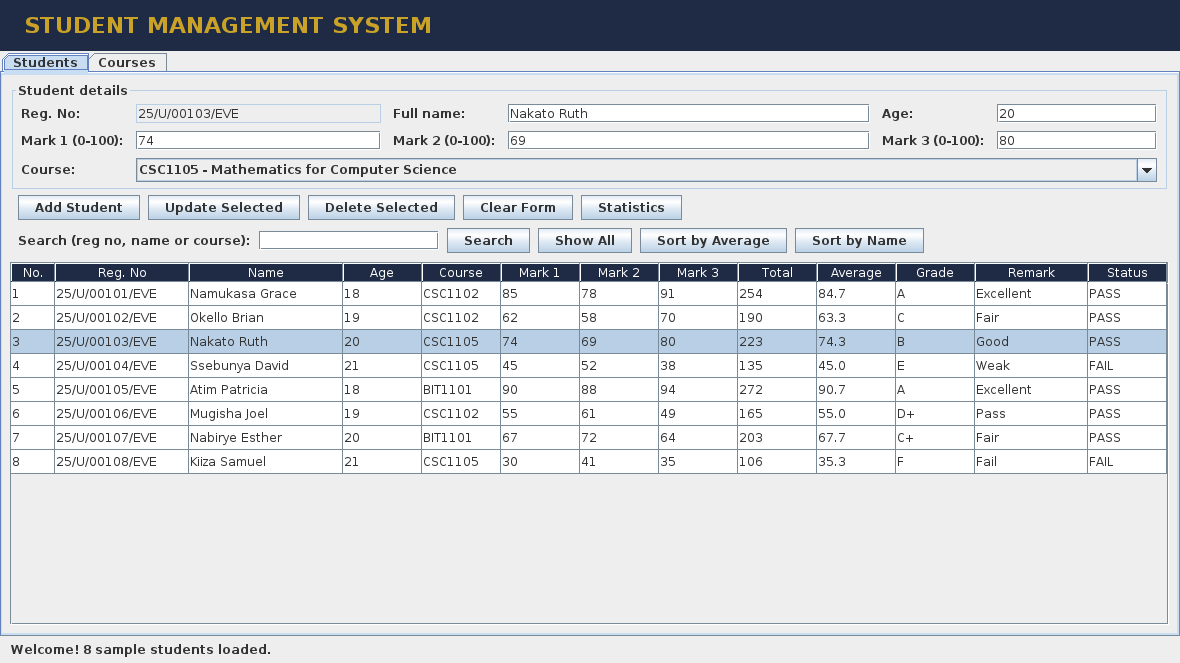
\includegraphics[width=0.68\textwidth]{images/gui_students.png}
    \caption{\textbf{Students Tab:} Live execution showing the student details form, action/search/sort buttons, and the student registry table with row 3 (\texttt{25/U/00103/EVE}, Nakato Ruth) selected and loaded into the form.}
    \label{fig:students_gui}
\end{figure}

\vspace{-0.15cm}
\begin{figure}[H]
    \centering
    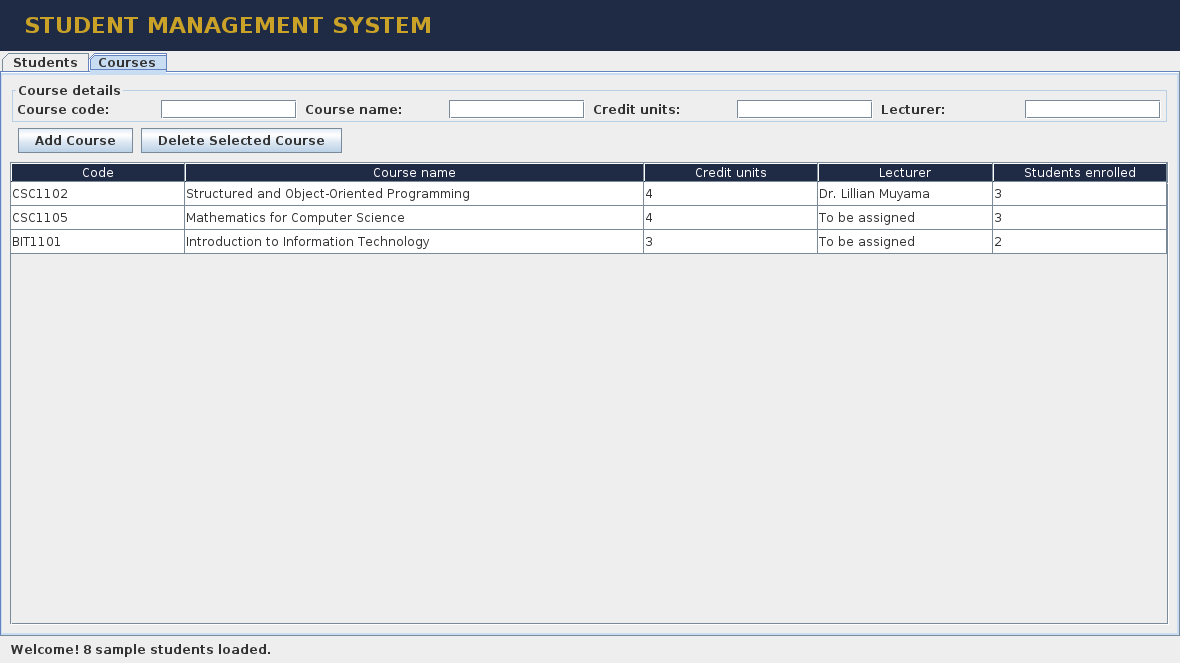
\includegraphics[width=0.68\textwidth]{images/gui_courses.png}
    \caption{\textbf{Courses Tab:} Live execution displaying course management controls and the course registry table with real-time enrolled student counts (\texttt{CSC1102}: 3, \texttt{CSC1105}: 3, \texttt{BIT1101}: 2).}
    \label{fig:courses_gui}
\end{figure}

\end{document}
